%!TEX root = ClementiCooperBarba2018.tex

\subsection{Isolated particle} \label{sec:verification}

In this section we present the results of performing a verification exercise. We
compare our numerical calculations of the extinction cross-section using boundary
elements method (BEM), with analytical solutions available for spherical geometries. 

The analytical expression for the extinction cross-section of spherical geometries
provided by Mishenko \cite{Mishchenko2007} applies for all mediums. In the presence
of a lossy medium, $k^\prime$ represents the real part of the complex wave number,
otherwise $k$ is a real-valued and we take $k^\prime = k$. 


\begin{equation} 
    C_\text{ext} = \frac{4\pi a^3}{k^\prime} \operatorname{Im}\left(k^2 
                    \frac{\epsilon_p/\epsilon_m -1}{\epsilon_p/\epsilon_m -2}\right)
    \label{eq:an_sol}
\end{equation}

where $a$ is the radius of the sphere, $k$ the complex wave number ($k=k^\prime +i k^{\prime\prime}$), $\epsilon_p$ 
the dielectric constant of the particle, and $\epsilon_m$ the dielectric constant
of the host medium. 

When we applied the electrostatic approximation, the simulations reduces to a 
sphere under a constant electric field, like presented in Fig. \ref{fig:np_elec_field}.

\begin{figure}[h] %  figure placement: here, top, bottom, or page
   \centering
   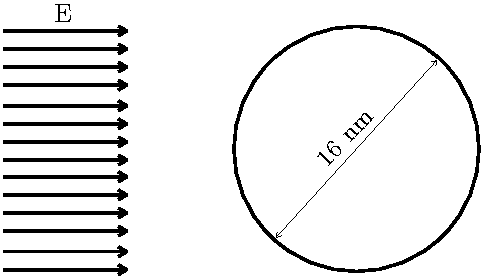
\includegraphics[width=0.3\textwidth]{sphere_field_8nm.pdf} 
   \caption{Spherical nanoparticle in a constant electric field.}
   \label{fig:np_elec_field}
\end{figure}

Figure \ref{fig:error_sphere_Ag} shows a grid convergence study of the extinction
cross-section of a silver spherical nanoparticle of radius $8 \, nm$ inmersed in water
under a z-polarized electric field with a wavelength of $380 nm$ and intensity of 
$-0.0037 e/({\AA}^2 \, \epsilon_0)$. Under these conditions water has a dielectric
constant of $1.7972 \, + \, 8.5048^{-09}i$ \cite{JohnsonChristy1972} and silver of
$-3.3877 \, + \, 0.1922i$ \cite{HaleQuerry1972}. In these simulations we used $K=4$ 
Gauss quadrature points per far-away elements, $K_fine = 37$ Gauss quadrature points
per elements for near singular integrals, $Nk = 9$ Gauss quadrature points per 
triangle edge for semi-analytical integration in the singular elements, and a GMRES
tolerance of $10^{-5}$. We performed the simulation for meshes of 512, 
2048, 8192 and 32768 elements. The error calculation uses the analytical solution 
$C_{ext} = 1854.4765 \; nm^2$ obtained using equation \eqref{eq:an_sol}.

\begin{figure}[h] %  figure placement: here, top, bottom, or page
   \centering
   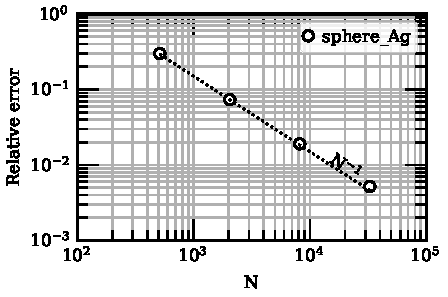
\includegraphics[width=0.45\textwidth]{convergence_sph_Ag_R8_w=380.pdf} 
   \caption{Grid-convergence study of extinction cross-section of a spherical silver
            nanoparticle.}
   \label{fig:error_sphere_Ag}
\end{figure}

The computed order of converge is $0.98$ and the $1/N$ slope in Fig. \ref{fig:error_sphere_Ag}
show that the numerical solutions computed with \pygbe for isolated spheres are
correctly resolved by the meshes.

The percentage errors for the different meshes are presented in the following table:

\begin{table}[h]
    \centering
    \caption{\label{table:err_iso_sphere} Percentage error of isolated silver sphere.} 
    \begin{tabular}{c c}
    \hline%\toprule
    N & \% error \\
    \hline%\midrule
     $512$ & $29.86$ \\
     $2048$ & $7.33$ \\
     $8192$ & $1.9$ \\
     $32768$ & $0.52$ \\
    \hline%\bottomrule
    \end{tabular}
\end{table}



\begin{figure}[h] %  figure placement: here, top, bottom, or page
   \centering
   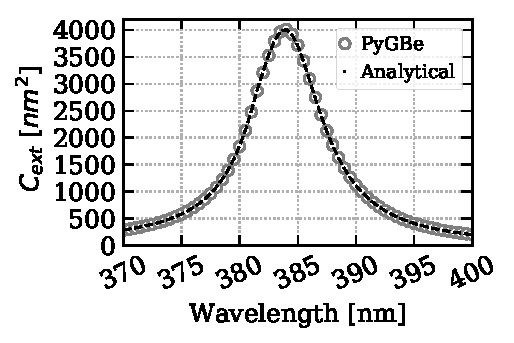
\includegraphics[width=0.45\textwidth]{silver_NP_verification.pdf} 
   \caption{Verification performed by comparing our numerical calculations of 
            the extinction cross-section with analytical solutions, available 
            for spherical geometries. We compare our results against the analytical
            solution provided by Mishenko \cite{Mishchenko2007} which applies for all mediums.
            In our case the medium is water and treated as a lossy medium. We can
            see good agreement between simulations and analytical results, proving
            that we are achieving an accurate numerical solution of the mathematical
            model.}
   \label{fig:verif_sphere}
\end{figure}

\subsection{Silver nanoparticle response to BSA} \label{sec:verification}


\begin{figure}[h] %  figure placement: here, top, bottom, or page
   \centering
   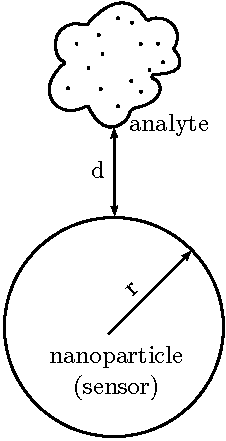
\includegraphics[width=0.15\textwidth]{protein_sphere_sketch.pdf} 
   \caption{Setup for convergence analysis of the response calculation}
   \label{fig:setup_conv}
\end{figure}


Convergence analysis for system sensor-BSA


\begin{figure}[h] %  figure placement: here, top, bottom, or page
   \centering
   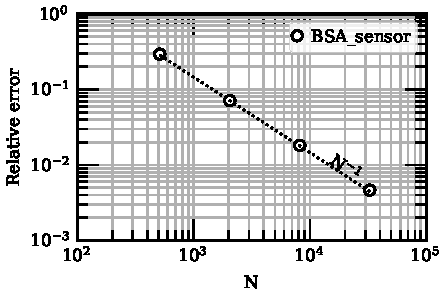
\includegraphics[width=0.45\textwidth]{convergence_bsa_sensor_R8_d=1_w=380.pdf} 
   \caption{Grid-convergence study for the silver spherical nanoparticle 
            response to Bovine Serum Albumina (BSA). We performed the 
            mesh-refinement on the sensor (silver nanoparticle) since this is 
            the surface where the extinction cross section is computed. We run
            the case presented in \ref{fig:display_z} for radius of
            the sphere of 8nm, a wavelength of  380 nm and a distance $d=1nm$
            along the z-axis, for sensor-meshes of 512, 2048, 8192 and 32768 
            elements. The error calculation uses the Richardson extrapolation 
            value of the extinction cross section as a reference 
            $C_{ext} = 1778.7259 \; nm^2$, computed using the 3 finner meshes.}
   \label{fig:error_sphere-bsa}
\end{figure}


We can see in Figure \ref{fig:error_sphere-bsa} the error decays with number
of boundary elements ($\frac{1}{N}$), which is consistent with our verification 
results (reference verification convergence figure). This proves that the
numerical solutions computed with \pygbe are correctly resolved by the meshes. 



\begin{figure*}[h] %  figure placement: here, top, bottom, or page
   \centering
   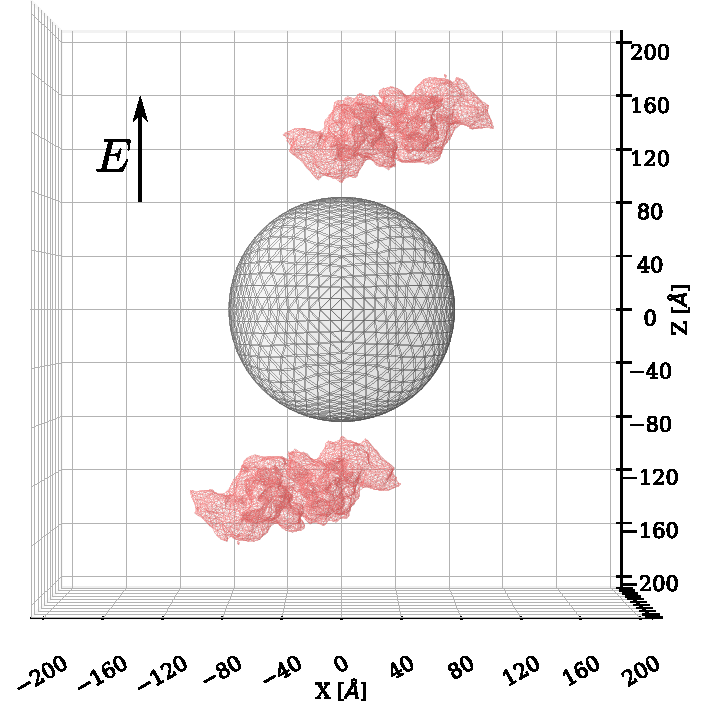
\includegraphics[width=0.5\textwidth]{2prot_1nm_z_R8nm.pdf} 
   \caption{Sensor protein display: BSA located at 1 nm of the nanoparticle in the
            z-direction}
   \label{fig:display_z}
\end{figure*}


Fig result of 2pz based on distance

\begin{figure}[h] %  figure placement: here, top, bottom, or page
   \centering
   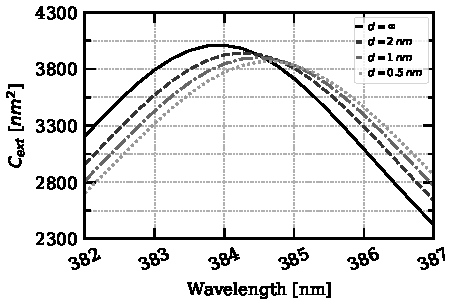
\includegraphics[width=0.45\textwidth]{2pz_lspr_response.pdf} 
   \caption{}
   \label{fig:dist_response}
\end{figure}



Fig result of 2pz

\begin{figure}[h] %  figure placement: here, top, bottom, or page
   \centering
    %since we have dots in the names we need to enclose what is before the 
    %extension in { }
   \includegraphics[width=0.45\textwidth]{{2pz_00_ef-0.0037_R8nm}.pdf} 
   \caption{}
   \label{fig:2pz_response}
\end{figure}



\begin{figure*}[h]

   \centering
   \subfloat{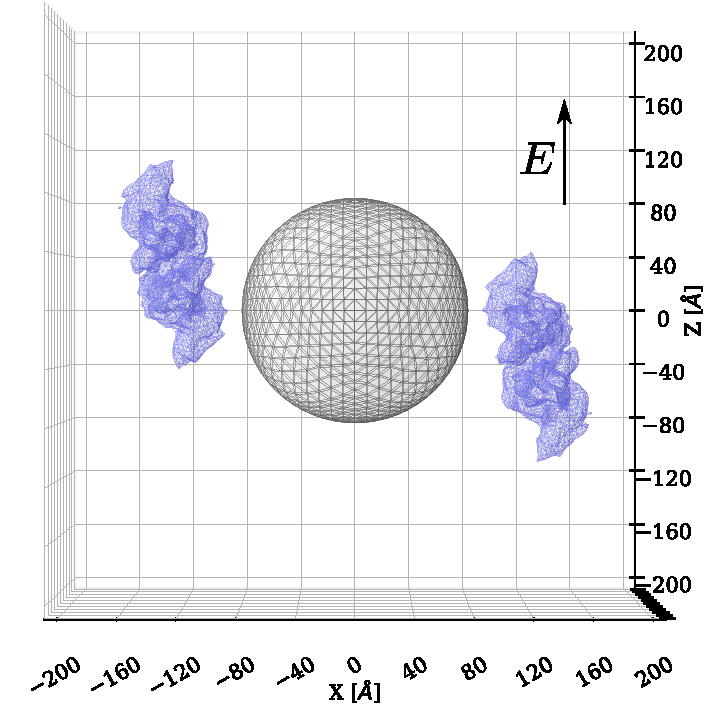
\includegraphics[width=0.49\textwidth]{2prot_1nm_x_R8nm.pdf}} 
%   \caption{Sensor protein display: BSA located at 1 nm of the nanoparticle in the
%            x-direction}
   %\label{fig:display_x}
    \quad
   \subfloat{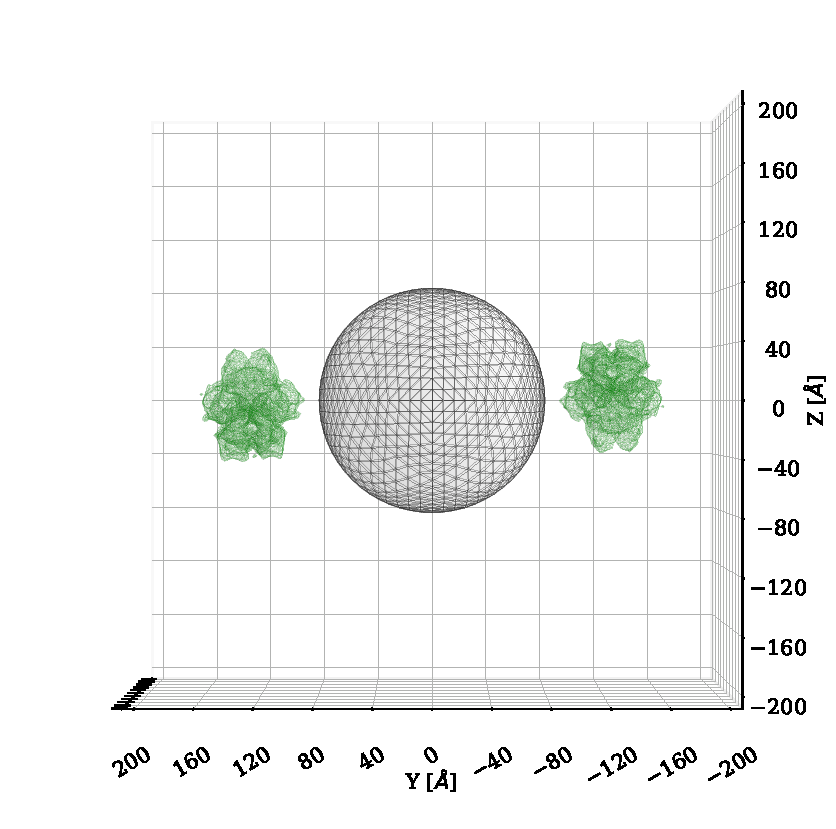
\includegraphics[width=0.49\textwidth]{2prot_1nm_y_R8nm.pdf}} 
%   \caption{Sensor protein display: BSA located at 1 nm of the nanoparticle in the
%            y-direction}
   \label{fig:display_y}
    \caption{Sensor protein display: BSA located at 1 nm of the nanoparticle in the
            x-direction (left) and y-direction (right)}

\end{figure*}


the variation of the extinction cross-section with respect to the wavelength, for each of the distances shown above. The red shift in the resonance frequency and the decrement of the peak in the presence of the analyte agrees with the behavior observed in experiments perform by Tang et al. \cite{TangETal2010}. This indicates that our boundary element method approach, using electrostatic approximation, is capable of reproducing characteristic resonance frequency shift in LSPR biosensors.




Experiments suggests that the distance between the nanoparticle and the analyte affects the sensitivity of the sensor \cite{HaesETal2004}, and these proof-of-concept calculations show that our approach can be use to study sensitivity versus distance, using electrostatics.




Generate distance variation plot. 


Fig result of 2px and 2py

\begin{figure}[h] %  figure placement: here, top, bottom, or page
   \centering
   \includegraphics[width=0.45\textwidth]{{2px_00_ef-0.0037_R8nm}.pdf} 
   \caption{}
   \label{fig:2px_response}
\end{figure}

\begin{figure}[h] %  figure placement: here, top, bottom, or page
   \centering
   \includegraphics[width=0.45\textwidth]{{2py_00_ef-0.0037_R8nm}.pdf} 
   \caption{}
   \label{fig:2py_response}
\end{figure}



